\chapter{Śledzenie obiektów w sekwencjach obrazów}
\label{cha:Sledzenie_obiektow_w_sekwencjach_obrazow}

\section{Wprowadzenie}
\label{sec:Sledzenie_obiektow_w_sekwencjach_obrazow_wprowadzenie}
Śledzenie obiektów w sekwencjach obrazów stanowi funkcję licznej grupy zróżnicowanych algorytmów przetwarzania obrazów, o wielu praktycznych zastosowaniach, wśród których można wymienić \cite{Yilmaz2006}:

\begin{itemize}

	\item Wykrywanie obiektów na obrazie w oparciu o ich ruch
	\item Automatyczny monitoring (ang. \textit{video surveillance}), tzn. wykrywanie i rejestrację podejrzanych zdarzeń
	\item Indeksację sekwencji video, tzn. ich oznaczanie i klasyfikację ich fragmentów
	\item Tworzenie interfejsów człowiek-komputer, poprzez rozpoznawanie gestów, okulografię, etc.
	\item Monitorowanie ruchu ulicznego, tzn. automatyczne gromadzenie danych statystycznych na temat jego natężenia
	\item Nawigację pojazdów, tzn. planowanie trasy oraz unikanie kolizji w oparciu o obraz z kamery video

\end{itemize}	
	
Śledzenie obiektów można zdefiniować jako estymację ich trajektorii na  płaszczyźnie obrazu, lub ich spójne etykietowanie na kolejnych klatkach sekwencji video. Opcjonalnie, algorytm może również dostarczać informacji o cechach samego obiektu, np. jego orientacji, rozmiarze, czy kształcie \cite{Yilmaz2006}. Tak określone zadanie w ogólnym ujęciu jest skomplikowane ze względu na szereg utrudniających je zjawisk, występujących w rzeczywistych sekwencjach video, takich jak \cite{Yilmaz2006}:

\begin{itemize}

	\item Utrata części informacji o obiekcie, wynikająca z projekcji trójwymiarowej rzeczywistości na dwuwymiarową płaszczyznę obrazu
	\item Zakłócenia występujące na obrazach rejestrowanych kamerą
	\item Skomplikowany charakter ruchu obiektów zainteresowania
	\item Brak spełniania warunku sztywności obiektów zainteresowania
	\item Częściowe i całkowite przysłonięcia obiektów zainteresowania
	\item Złożony kształt obiektów  zainteresowania
	\item Zmiany oświetlenia sceny na obrazach
	\item Wymaganie czasu rzeczywistego obliczeń

\end{itemize}  

Samo zagadnienie od dawna stanowi przedmiot badań, w związku z czym powiązane z nim pojęcia i problemy są dokładnie sklasyfikowane i zdefiniowane, zaś dotycząca go literatura jest bardzo obszerna. Tym niemniej ze względu na jego trudność opracowane dotychczas rozwiązania cechują się specjalizacją, tj. wykazują odporność na część z przedstawionych wyżej problemów, przy jednoczesnym jej braku na pozostałe \cite{Smeulders2010}.

\section{Ogólny model algorytmów śledzenia obiektów na obrazach}
\label{sec:Ogolny_model_algorytmow_sledzenia_obiektow_na_obrazach}

Choć algorytmy śledzenia obiektów na obrazach są bardzo zróżnicowane, można dokonać ich dekompozycji na pięć podstawowych etapów \cite{Smeulders2010}:

\begin{itemize}
	\item Określenie obszaru występowania obiektu zainteresowania
	\item Wyznaczenie reprezentacji obiektu zainteresowania
	\item Wyznaczenie modelu ruchu obiektu zainteresowania
	\item Wykonanie pomiaru podobieństwa oraz określenie dopasowania obiektu pomiędzy kolejnymi klatkami sekwencji obrazów
	\item Uaktualnienie reprezentacji obiektu zainteresowania
\end{itemize}
 
Na rysunku \ref{fig:Ogolny_model_dzialania_algorytmow_sledzenia_obiektow} przedstawiono schemat kolejności realizacji tych etapów. Nie uwzględnia on fazy wykrywania obiektu, stanowiącej odrębne zagadnienie cyfrowego przetwarzania obrazów, omówione w rozdziale \ref{cha:Wykrywanie_poruszajacych_sie_obiektow}.

\begin{figure}[!htb]
	\begin{center}
		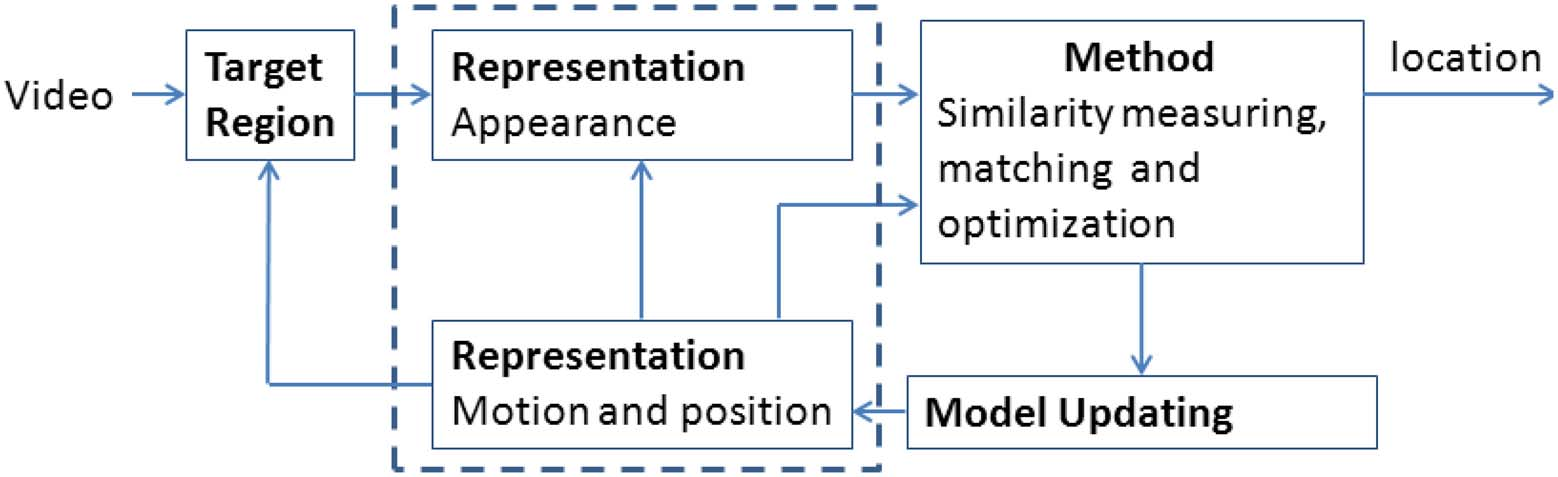
\includegraphics[width=12cm]{images/object_trackers_reference_model.png}
	\end{center}	
	\longcaptionsource{Ogólny model działania algorytmów śledzenia obiektów w sekwencjach video}{\textit{Target region} - Obszar zainteresowania (obszar obrazu zawierający obiekt zainteresowania)\\\textit{Representation - appearance} - Model  obiektu zainteresowania określający jego cechy charakterystyczne\\\textit{Representation - motion and position} - Model ruchu obiektu zainteresowania\\\textit{Method - similarity measuring, matching and optimization} - metoda pomiaru podobieństwa oraz stwierdzenia dopasowania obiektu pomiędzy klatkami\\\textit{Model updating} - metoda aktualizowania modelu cech obiektu zainteresowania	
}{\cite{Smeulders2010}}
\label{fig:Ogolny_model_dzialania_algorytmow_sledzenia_obiektow}
\end{figure}

\subsection{Reprezentacje obiektu na obrazie}
\label{subsec:Reprezentacje_obiektu_na_obrazie}

Pierwszym krokiem po uzyskaniu informacji o wystąpieniu obiektu jest zdefiniowanie jego reprezentacji rozumianej tutaj jako wyodrębnione składowe elementy obrazu przynależące do tego obiektu.

W najprostszym przypadku obiekt przybliża się jego \textbf{bryłą brzegową}, o postaci prostokąta lub elipsy zawierającej wszystkie należące do niego piksele. Inaczej mówiąc reprezentację obiektu stanowi fragment obrazu, który go zawiera. Zaletą takiego rozwiązania jest minimalna liczba parametrów opisująca obiekt, wadą natomiast włączeniem do jego reprezentacji dużej liczby pikseli tła \cite{Smeulders2010}.

Pewnym ulepszeniem tej koncepcji, zwiększającym jej odporność, jest stosowanie \textbf{wielu brył brzegowych} jednocześnie. Takie rozwiązanie cechuje się również większą elastycznością w dalszych krokach algorytmu, w których realizowane jest poszukiwane położenia w kolejnej klatce (uproszczone w przypadku pojedynczej bryły brzegowej do jednego punktu) \cite{Smeulders2010}.

Inną możliwą, lecz rzadko stosowaną w tej rodzinie algorytmów reprezentacją jest \textbf{kontur} obiektu zainteresowania. Cechuje się ona małą rygorystycznością w stosunku do zmiany ogólnego wyglądu obiektu, jednak jej użycie jest ograniczone do przypadków, w których stosowanie deskryptorów kształtu zapewnia wysoką dokładność \cite{Smeulders2010}.

Pozornie podobny sposób reprezentacji polega na określeniu \textbf{ciągłego obszaru obrazu} zawierającego piksele należące do obiektu zainteresowania. Należy zwrócić uwagę, że taka reprezentacja obiektu nie jest równoznaczna jego sylwetce (ang. \textit{silhouette}), rozumianej jako sumę zbiorów pikseli konturu obiektu oraz zbioru pikseli zawartych wewnątrz wyznaczonej przez niego bryły. Różnica ta jest wynikiem sposobu wyznaczania tych dwóch reprezentacji. Przedstawienie obiektu w postaci ciągłego obszaru obrazu pozwala na jego precyzyjne oddzielnie od innych obiektów. Wymaga natomiast dużej odporności od metody jego wyznaczenia, w celu uniknięcia wniesienia błędnej informacji o samym obiekcie \cite{Smeulders2010}.  

Nieco bardziej złożona reprezentacja obiektu oparta jest jest o \textbf{skrawki obrazu}. Są to małe obszary obrazu zawierające fragmenty obiektu zainteresowania, którego wygląd może zmieniać się niezależnie w ich obrębie. Odmianą tego modelu jest reprezentacja w postaci punktów charakterystycznych (ang. \textit{sailent points} lub \textit{interest points}), w których występuje pewna cecha charakterystyczna (ang. \textit{feature}) obrazu. Istnieją różne koncepcje definicji zbioru oraz relacji pomiędzy skrawkami obrazu \cite{Smeulders2010}. Cechą charakterystyczną takiej reprezentacji jest brak konieczności wyraźnego rozróżnienia pomiędzy tłem a obiektem zainteresowania. Skutkuje ona zwiększoną odpornością na przysłonięcia oraz zmianę kształtu obiektu zainteresowania. Z drugiej strony, w przypadku małych lub sztywnych obiektów reprezentacja skrawkami obrazu nie jest bardziej wydajna od reprezentacji opierających się o zbiory pojedynczych pikseli (jak np. w postaci bryły brzegowej) \cite{Smeulders2010}.

Na rysunku \ref{fig:Reprezentacje_obiektu_na_obrazie} przedstawiono przykładowy obiekt zainteresowania oraz wizualizacje odpowiadających mu reprezentacje według omówionych koncepcji.

\begin{figure}[!htb]
	\begin{center}
		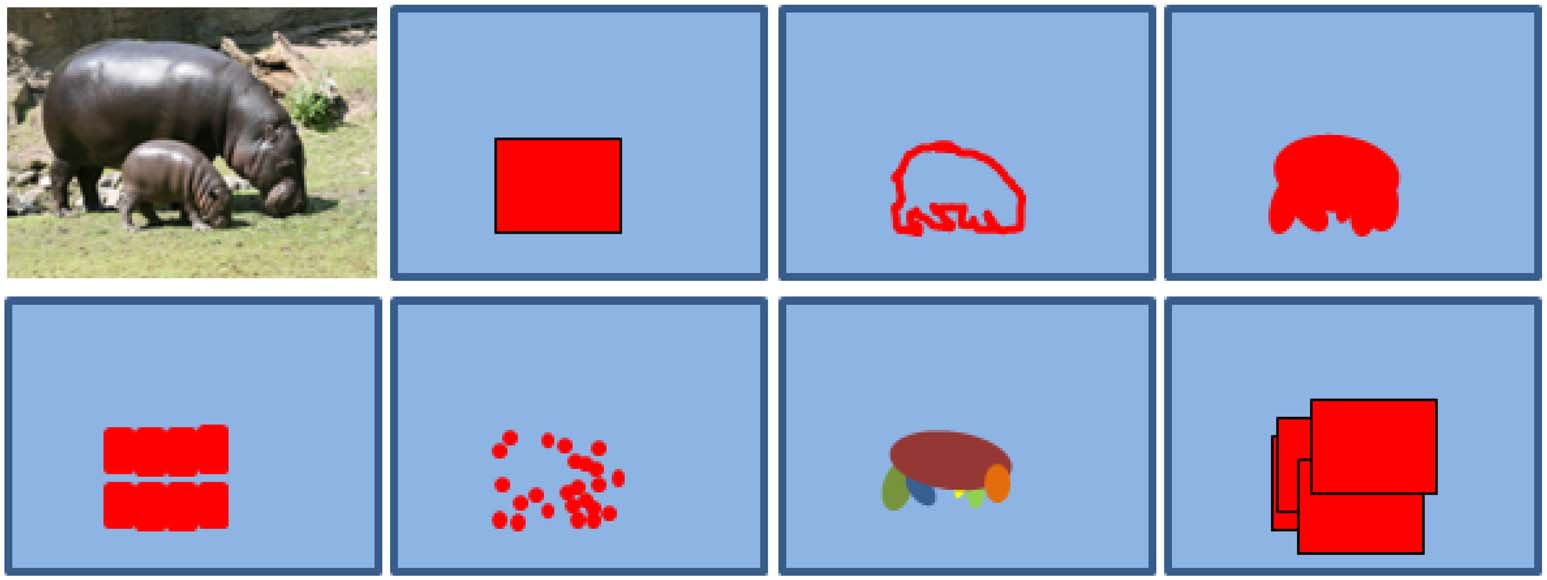
\includegraphics[width=12cm]{images/target_region_representation.png}
	\end{center}	
	\longcaptionsource{Reprezentacje obiektu zainteresowania na obrazie}{Kolejno, od lewego górnego rogu: obraz wejściowy, bryła brzegowa (ang. \textit{bounding box}), kontur obiektu, obszar obiektu (ang. \textit{blob}), skrawki obrazu (ang. \textit{image patches}), rozproszony zbiór punktów zainteresowania, części obiektu, wiele brył brzegowych}{\cite{Smeulders2010}}
\label{fig:Reprezentacje_obiektu_na_obrazie}
\end{figure}

\subsection{Modele obiektu zainteresowania}
\label{subsec:Modele_obiektu_zainteresowania}

Model obiektu, rozumiany jako opis jego cech charakterystycznych, tworzony jest w obrębie zdefiniowanego wcześniej obszaru zainteresowania (\ref{subsec:Reprezentacje_obiektu_na_obrazie}). Podstawowym wymaganiem, które musi spełniać jest zdolność do zachowania określonej właściwości pomiędzy kolejnymi klatkami, bez której wykonanie zadania śledzenia obiektu nie jest możliwe \cite{Smeulders2010}.

Istnieją trzy podstawowe reprezentacje cech charakterystycznych obiektu stosowane w algorytmach śledzenia: dwuwymiarowa tablica wartości pikseli, histogram oraz wektor cech \cite{Smeulders2010}.

Najbardziej oczywistą i bezpośrednią jest reprezentacja w postaci \textbf{dwuwymiarowej tablicy wartości pikseli obiektu} (rysunek \ref{fig:Modele_obiektu_zainteresowania}a). Najczęściej w tablicy przechowywane są wartości określające jasności poszczególnych pikseli \cite{Smeulders2010}, pomimo idącego za tym założenia dotyczącego jej stałych wartości, które rzadko jest prawdziwe. Tym niemniej taka reprezentacja nie powoduje utraty informacji o obiekcie wewnątrz obszaru zainteresowania.

Reprezentacja w postaci \textbf{histogramu} (rysunek \ref{fig:Modele_obiektu_zainteresowania}b) wyznaczana jest najczęściej w oparciu kolor pikseli w obszarze zainteresowania, występuje również w wersji przechowującej jedynie ich jasności \cite{Smeulders2010}. Przy reprezentacji w tej postaci następuje całkowita utrata informacji o właściwościach przestrzennych obiektu, przechowywana jest jedynie informacja o wartościach poszczególnych pikseli, co skutkuje największą elastycznością w odniesieniu do zmiany kształtu obiektu \cite{Smeulders2010}.

Reprezentacja w postaci \textbf{wektora cech} (rysunek \ref{fig:Modele_obiektu_zainteresowania}c) polega na wykryciu oraz deskrypcji cech charakterystycznych obiektu (ang. \textit{features}). W jej przypadku również nie przechowuje się informacji o kształcie geometrycznym obiektu \cite{Smeulders2010}. Cechy wraz z ich deskryptorami odwzorowują obiekt w oparciu o jego najbardziej bogate w informację właściwości, pozwalając na ograniczenie rozmiaru jego reprezentacji \cite{Smeulders2010}.

\begin{figure}[!htb]
	\begin{center}
		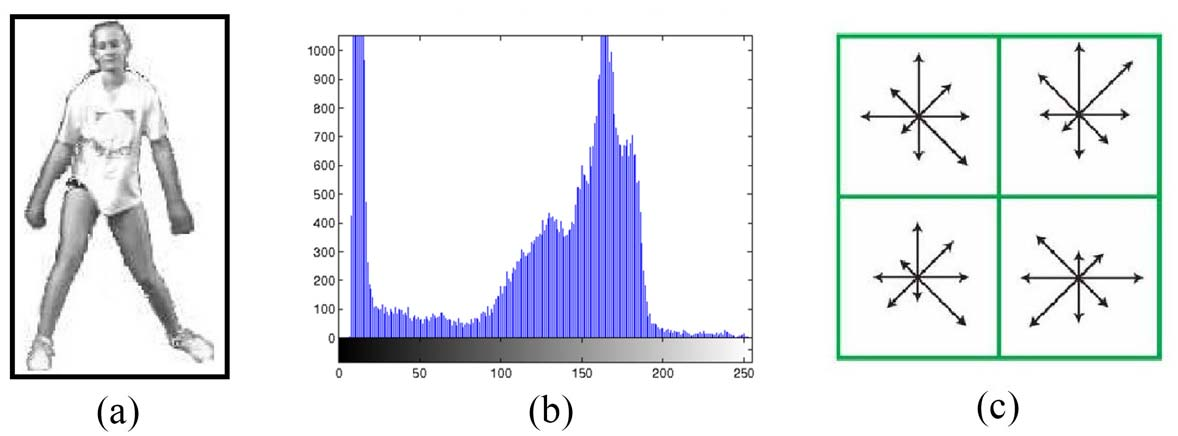
\includegraphics[width=12cm]{images/target_appearance_representation.png}
	\end{center}	
	\longcaptionsource{Modele obiektu zainteresowania, stosowane w algorytmach śledzenia obiektów}{a) Tablica dwuwymiarowa b) Histogram c) Wektor cech}{\cite{Smeulders2010}}
\label{fig:Modele_obiektu_zainteresowania}
\end{figure}

\subsection{Modele ruchu obiektu}
\label{subsec:Modele_ruchu_obiektu}

Przyjęcie założeń dotyczących ruchu obiektu (w tym sensie, stworzenie jego uproszczonego modelu) ma za zadanie zawężenie okna, w którym następuje próba stwierdzenia wystąpienia obiektu na kolejnej klatce sekwencji.

Najprostszy model nie narzuca żadnych ograniczeń poza założeniem, że obiekt po wykonaniu przemieszczenia pomiędzy kolejnymi klatkami znajduje się blisko pozycji początkowej \cite{Smeulders2010}. Jego implikacją jest stwierdzenie możliwości lokalizacji kolejnego położenia obiektu poprzez przeszukanie małego okna wokół poprzedniego \cite{Smeulders2010}, skąd nazwa \textbf{przeszukiwanie jednorodne}. Dzięki braku założeń dotyczących charakteru samego ruchu, rozwiązanie to cechuje duża ogólna odporność, nie sprawdza się ono jednak, jeśli ruch obiektu jest szybki \cite{Smeulders2010}.

Rozwinięciem koncepcji opisanej wyżej jest \textbf{gaussowski model ruchu}, w którym wprowadza prawdopodobieństwo wystąpienia kolejnego położenia obiektu wokół położenia początkowego zmienia się zgodnie z rozkładem normalnym. W tej reprezentacji dopasowaniu obiektu na kolejnej klatce przypisywany jest dodatkowo współczynnik wagowy (w oparciu o prawdopodobieństwo), co pozwala na zwiększenie przestrzeni poszukiwania \cite{Smeulders2010}.

Innym możliwym modelem jest \textbf{predykcja ruchu} obiektu z wykorzystaniem jego liniowego modelu oraz filtru Kalmana \cite{Smeulders2010}. Taką reprezentację można dodatkowo ulepszyć, wykonując predykcję w oparciu o przepływ optyczny \cite{Smeulders2010}.

W \textbf{bezpośredniej predykcji ruchu} nie przyjmuje się założeń odnośnie modelu ruchu, wykorzystuje się natomiast metody optymalizacji do znalezienia najlepiej dopasowanego nowego położenia w oparciu o położenia występujące wcześniej \cite{Smeulders2010}. Taki model jest jednak mało użyteczny, ponieważ wymaga, aby przemieszczenia obiektu były małe w porównaniu do innych zmian występujących na obrazie \cite{Smeulders2010}.

Ostatnia z metod reprezentacji polega na równoległym \textbf{śledzeniu i detekcji} obiektu z zastosowaniem niezależnych algorytmów. Po takim podejściu można oczekiwać dużej odporności na przypadkowe ruchu zarówno obiektu jak i kamery \cite{Smeulders2010}, jednak cechuje się ono największą komplikacją.

Na rysunku \ref{fig:Modele_ruchu_obiektu} zestawiono i porównano przedstawione wyżej sposoby modelowania ruchu. 

\begin{figure}[!htb]
	\begin{center}
		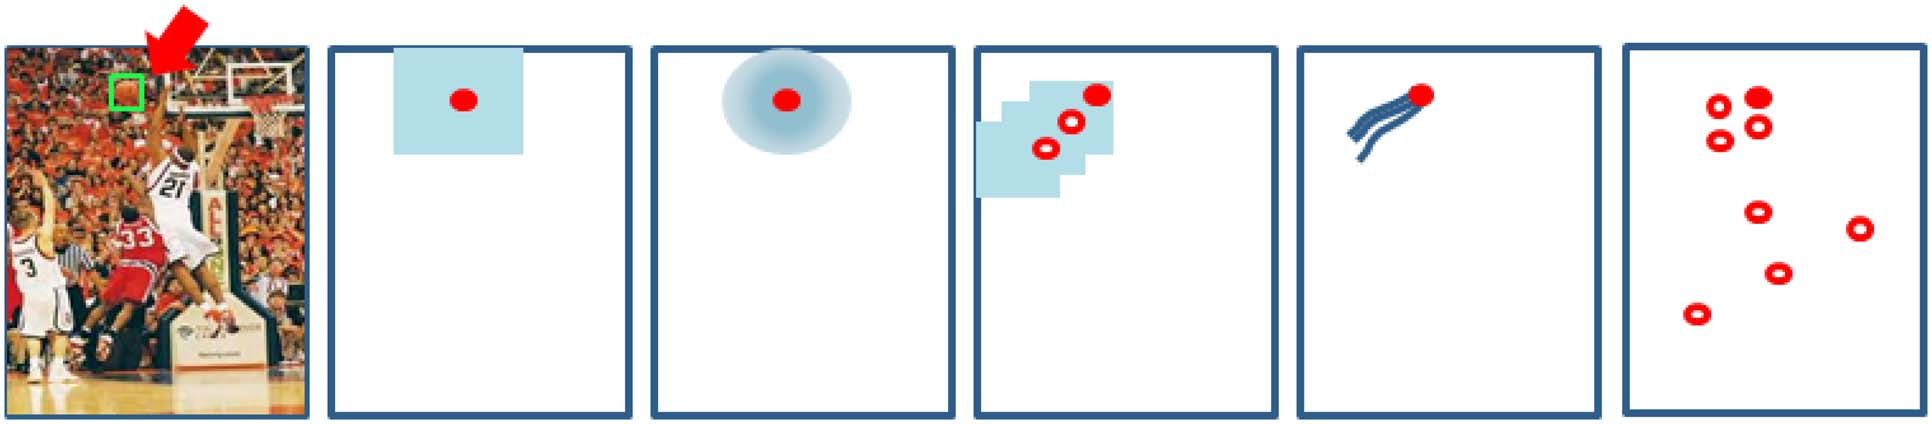
\includegraphics[width=12cm]{images/target_motion_representation.png}
	\end{center}	
	\longcaptionsource{Modele ruchu obiektu, stosowane w algorytmach śledzenia obiektów}{Od lewej: obiekt zainteresowania, przeszukiwanie jednorodne, gaussowski model ruchu, predykcja ruchu, model wprost, śledzenie i wykrywanie}{\cite{Smeulders2010}}
\label{fig:Modele_ruchu_obiektu}
\end{figure}

\subsection{Metody pomiaru podobieństwa oraz stwierdzenia dopasowania obiektu pomiędzy klatkami}
\label{subsec:Metody_pomiaru_podobienstwa_oraz_stwierdzenia_dopasowania_obiektu pomiedzy_klatkami}

Metoda pomiaru podobieństwa obiektu oraz stwierdzenia jego dopasowania pomiędzy klatkami to kluczowy element algorytmu śledzenia, które w tym właśnie etapie jest zasadniczo realizowane.

Pierwsza i najprostsza jej realizacja opiera się na wykonaniu \textbf{dopasowania} pomiędzy znanym modelem obiektu zainteresowania na początkowej klatce, do kandydatów, których modele tworzone są dla jego możliwych położeń na kolejnej klatce, zgodnie z przyjętym modelem ruchu. Jednemu znanemu obiektowi zainteresowania jest więc przypisywany zbiór jego możliwych kolejnych instancji (rysunek \ref{fig:Metody_sledzenia_obiektow_na_obrazach}a), spośród których wybierana jest najlepiej dopasowana.
Inaczej mówiąc, śledzenie w tym przypadku jest zdaniem optymalizacji. Na podstawie podejścia do jego rozwiązania można wyróżnić dwie kategorie - dopasowanie bezpośrednie, polegające na poszukiwaniu najlepszego kandydata wzdłuż gradientu pewnej funkcji określającej dopasowanie, oraz dopasowanie probabilistyczne, polegające na znalezieniu maksimum funkcji gęstości prawdopodobieństwa, opisującej prawdopodobieństwo wystąpienia obiekt zainteresowania w danych punkcie obrazu. Dopasowanie bezpośrednie wykazuje dużą odporność przy wielu różnych modelach ruchu obiektu, przy zachowaniu warunku małej przestrzeni przeszukiwania. Z drugiej strony opiera się one o silne założenia dotyczące opisu modelu obiektu, w skutek jest wrażliwe na lokalne zmiany intensywności pikseli (występujące w rzeczywistych sekwencjach obrazów, w wyniku np. zmiany kąta padania światła) oraz jakość reprezentacji obiektu na obrazie \cite{Smeulders2010}. Dopasowanie probabilistyczne jest efektywne w przypadku możliwości wystąpienia przysłonięcia obiektu oraz niejednoznaczności, pojawiających się np. przy wielu podobnych obiektach \cite{Smeulders2010}.

\textbf{Dopasowanie z rozszerzonym opisem cech} rozszerza koncepcję dopasowania o opis modelu lub stan metody w przeszłości (dla ciągu przednich klatek) \cite{Smeulders2010}. Przy takim podejściu wieloelementowemu zbiorowi znanych wystąpień obiektu zainteresowania w ciągu poprzednich klatek przyporządkowywany jest wieloelementowy zbiorów kandydatów nowej instancji tego obiektu na klatce bieżącej (rysunek \ref{fig:Metody_sledzenia_obiektow_na_obrazach}b). Metoda przechowuje długotrwale trajektorię stanu obiektu zainteresowania, w związku z czym jest użyteczne w zadaniach śledzenia długoterminowego oraz w przypadku możliwości wystąpienia przysłonięć \cite{Smeulders2010}. Dopasowywanie jest wykonywane pomiędzy poszczególnymi elementami obydwu zbiorów, co skutkuje zwiększeniem złożoności obliczeniowej. 

W celu jej ograniczenia wprowadzono \textbf{dopasowywanie z więzami}, przy którym podobieństwo pomiędzy zbiorami wystąpień i kandydatów jest rozpatrywane jedynie dla elementów spełniających zdefiniowane kryteria, lub inaczej, więzy (rysunek \ref{fig:Metody_sledzenia_obiektow_na_obrazach}c). Mogą dotyczyć one, np. zmiany koloru lub kształtu obiektu pomiędzy kolejnymi klatkami. Metody tego typu mogą dobrze sprawdzać się w warunkach dużej zmienności obserwowanej sceny, nadają się również do zastosowania w algorytmach śledzących predefiniowanych wzorców \cite{Smeulders2010}.

Alternatywą dla metod opierających się o dopasowanie jest \textbf{klasyfikacja rozróżniająca}, określana inaczej jako ,,śledzenie przez wykrywanie'' \cite{Smeulders2010}. Opiera się ona o założenie, że samo odróżnienie pojedynczego obiektu zainteresowania od tła jest wystarczające do jego śledzenia \cite{Smeulders2010}. Klasyfikacja rozróżniająca polega więc na określeniu przynależności wszystkich pikseli obrazu do tła bądź obiektu zainteresowania, oraz uaktualnianiu informacji o tej przynależności na kolejnych klatkach sekwencji video. W tej metodzie występuje więc przyporządkowanie pomiędzy oznaczonym obiektem zainteresowania i jego tłem poprzedniej klatce oraz zbiorem par kandydat-tło na kolejnej (rysunek \ref{fig:Metody_sledzenia_obiektow_na_obrazach}d). Klasyfikator może przetwarzać zestaw wielu różnych cech jednocześnie, co pozwala na osiągnięcie dużej odporności w przypadku niskiej specjalizacji algorytmu śledzącego oraz wysokiej niestabilności obserwowanej sceny \cite{Smeulders2010}. U podstaw metody leży jednak domniemanie unikalności cech śledzonego obiektu w skali obrazu, co powoduje jej błędne działanie w przypadku jego wielokrotnego wystąpienia \cite{Smeulders2010}. Jest ona także wrażliwa na błędne etykietowanie pikseli, prowadzące do zakłócenia pracy klasyfikatora oraz przekłamania śledzonej trajektorii obiektu zainteresowania (ang. \textit{drift}).  

\textbf{Klasyfikacja rozróżniająca z więzami} jest rozwinięciem poprzedniej rodziny metod, wśród których główny nacisk kładzie się na poprawną klasyfikację i etykietowanie pikseli, a nie na poszukiwanie najlepszej (najbardziej dopasowanej lub prawdopodobnej) pozycji śledzonego obiektu \cite{Smeulders2010}. Polega ono na syntezie informacji o przynależności zbioru pikseli do obiektu z poszukiwaniem w jego otoczeniu obszaru najlepiej dopasowanego do stworzonego uprzednio modelu, w postaci np. wektora cech (rysunek \ref{fig:Metody_sledzenia_obiektow_na_obrazach}e). Wadą tej metody jest wysoka złożoność obliczeniowa, wynikająca ze stopnia jej komplikacji.

\begin{figure}[!htb]
	\begin{center}
		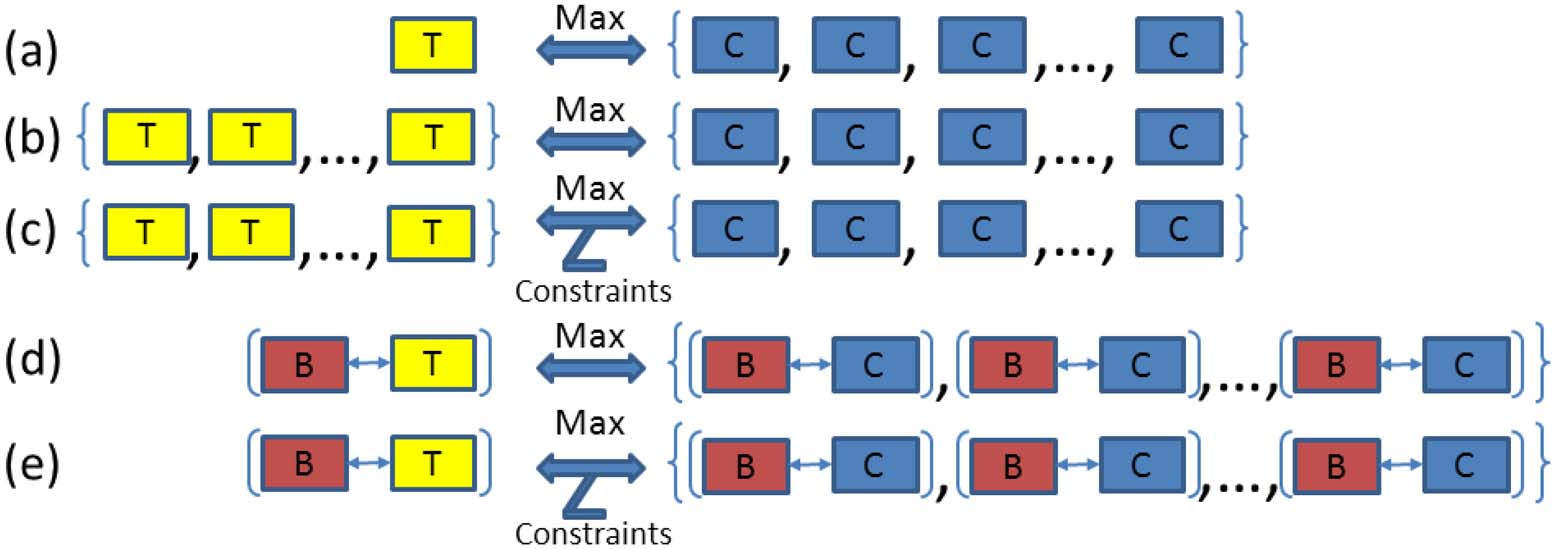
\includegraphics[width=12cm]{images/target_tracking_methods.png}
	\end{center}	
	\longcaptionsource{Metody śledzenia obiektów na obrazach}{a) Dopasowanie b) Dopasowanie z rozszerzonym opisem cech c) Dopasowanie z więzami d) Klasyfikacja rozróżniająca e) Klasyfikacja rozróżniająca z więzami. Oznaczenia bloków: T - wystąpienie obiektu zainteresowania, C - potencjalne kolejne wystąpienie obiektu zainteresowania, B - lokalne wystąpienia tła.}{\cite{Smeulders2010}}
\label{fig:Metody_sledzenia_obiektow_na_obrazach}
\end{figure}

\subsection{Metody uaktualnienia modelu obiektu zainteresowania}
\label{subsec:Metody_uaktualnienia_modelu_obiektu_zainteresowania}

Ostatni krok algorytmu śledzenia obiektu polega na uaktualnieniu stosowanego modelu na podstawie informacji zawartych w nowej klatce sekwencji video. W niektórych przypadkach nie jest on konieczny - poza uproszczeniem całego algorytmu, zaletą takiego rozwiązania jest brak wnoszenia błędnej informacji o obiekcie, która może być skutkiem niedoskonałego modelu \cite{Smeulders2010}.

Najprostsza realizacja uaktualnienia polega na \textbf{zastąpieniu} dotychczasowego opisu modelu opisem wykonanym dla ostatnio zaobserwowanego wystąpienia obiektu. Może się to odbywać w sposób częściowy, poprzez zastępowanie kolejnych fragmentów opisu nowymi, bądź przez okresowe, całościowe jego zastąpienie \cite{Smeulders2010}. 

\textbf{Predykcja} postaci modelu przy użyciu filtru Kalmana (\ref{sec:Filtr_Kalmana}) jest koncepcyjnie podobna, pozwalając jednocześnie na ograniczenie wpływu zakłóceń, zwłaszcza jeśli przebieg trajektorii obiektu jest łagodny. Gwałtowne jej zmiany skutkują jednak wniesieniem dodatkowego błędu \cite{Smeulders2010}. 

W przypadku reprezentacji obiektu w postaci skrawków obrazu, uaktualnianie modelu polega na odpowiednim ich wstawianiu, usuwaniu, zmienieniu i przesuwaniu. Jest to zadanie złożone, dodatkowo rozwiązywane w oparciu o ograniczony zasób informacji \cite{Smeulders2010}.

Dla algorytmów wykorzystujących rozszerzony opis cech obiektów stosowana jest przyrostowa analiza głównych składowych \cite{Smeulders2010}. Pozwala ona na przechowanie informacji o stanie modelu w przeszłości. 

\section{Śledzenie z wykorzystaniem przepływu optycznego}
\label{sec:Sledzenie_z_wykorzystaniem_przeplywu_optycznego}

\todo{Opis ogólnych wymagań w kontekście robotyki mobilnej - czas rzeczywisty, zmienne środowisko, etc.}

\subsection{Algorytm Lucasa-Kanade}
\label{subsec:Algorytm_Lucasa_Kanade}
Jak wspomniano wspomniano w podrozdziale \ref{subsec:Przeplyw_optyczny} analizę ruchu zarejestrowanego w sekwencji obrazów można przeprowadzić posługując się przepływem optycznym. Takie podejście znajduje zastosowanie w systemach wizyjnych przeznaczonych dla robotyki mobilnej. Szczególnie popularną metodą jego wyznaczania jest \textbf{algorytm Lucasa-Kanade}, został on wykorzystany w \cite{Markovic2014}, \cite{Sadeghi-Tehran2014}, \cite{Fernandez-Caballero2010}, \cite{Liem2008}.

Zastosowanie algorytmu Lucasa-Kanade wykracza znacznie poza zagadnienie śledzenia obiektów i obejmuje między innymi mozaikowanie obrazów, obrazowanie medyczne czy rozpoznawanie twarzy \cite{Baker2004}. Sam algorytm został po raz pierwszy opublikowany w roku 1981 i od tego czasu w literaturze zaproponowano szereg jego modyfikacji.

Oryginalnie funkcją pierwszej wersji algorytmu, nazywanej addytywną \cite{Baker2004}, było dopasowanie obrazu wzorcowego $T(\vec{x})$ do obrazu wejściowego $I(\vec{x})$, gdzie $\vec{x} = (x, y)^T$ jest wektorem współrzędnych pikseli. W przypadku wyznaczania przepływu optycznego, obraz wzorcowy $T(\vec{x})$ jest podregionem obrazu z sekwencji w chwili $t = 1$, natomiast $I(\vec{x})$ jest obrazem w chwili $t = 2$ \cite{Baker2004}. Zakłada się, że wzorzec $T(\vec{x})$ uległ na obrazie $I(\vec{x})$ pewnemu sparametryzowanemu odkształceniu (ang. \textit{warp}) $\matr{W}(\vec{x}, \vec{p})$, gdzie $\vec{p}$ jest wektorem parametrów. Odkształcenie $\matr{W}(\vec{x}, \vec{p})$ przyporządkowuje pikselom wzorca $T(\vec{x})$ ich subpikselowe położenie $W(\vec{x}, \vec{p})$ w układzie współrzędnych obrazu $I$  \cite{Baker2004}, przykład przedstawiono na rysunku \ref{fig:Algorytm_Lucasa_Kanade}. Odkształcenie pomiędzy dwoma kolejnymi obrazami w sekwencji, dla których wyznaczany jest przepływ optyczny ma postać \cite{Baker2004}:
\begin{equation}
\label{equ:Odksztalcenie_przeplyw_optyczny}
	\matr{W}(\vec{x}, \vec{p}) = \begin{bmatrix}
		x + p_1 \\
		y + p_2 \\
	\end{bmatrix}
\end{equation}

\noindent
gdzie:

\begin{conditions}
	\vec{p} = (p_1, p_2)^T & przepływ optyczny \\
\end{conditions}

Zasadniczym celem algorytmu jest minimalizacja sumy kwadratów błędów pomiędzy  wzorcem $T(\vec{x})$ a odkształconym obrazem wejściowym $I(W(\vec{x}, \vec{p}))$ \cite{Baker2004}:
\begin{equation}
\label{equ:Algorytm_Lucasa_Kanade_cel}
	\sum\limits_{\vec{x}} (I(\matr{W}(\vec{x}, \vec{p})) - T(\vec{x}))^2
\end{equation}

Ponieważ przekształcenie $\matr{W}(\vec{x}, \vec{p})$ zwraca wartości subpikselowe, do wyznaczenia wartości pikseli $I(\matr{W}(\vec{x}, \vec{p}))$ konieczne jest wykonanie ich interpolacji. Wyznaczenie przepływu optycznego sprowadza się do minimalizacji wyrażenia \ref{equ:Algorytm_Lucasa_Kanade_cel} , gdzie zmienną decyzyjną jest wektor $\vec{p}$. Takie zadanie optymalizacji ma charakter nieliniowy, ponieważ pomiędzy wartościami pikseli $I(\vec{x}$ a ich współrzędnymi $\vec{x}$ nie występuje zależność liniowa (ogólnie nie występuje żadna zależność) \cite{Baker2004}. Minimalizacja jest wykonywana iteracyjnie, poprzez założenie znajomości pewnej estymacji $p$ oraz wielokrotną zmianę jej wartości o $\Delta \vec{p}$ i wyznaczenie wartości błędu dla bieżącej postaci:
\begin{equation}
\label{equ:Algorytm_Lucasa_Kanade_iteracyjnie}
	\sum\limits_{\vec{x}} (I(\matr{W}(\vec{x}, \vec{p} + \Delta \vec{p})) - T(\vec{x}))^2
\end{equation}

\begin{equation}
\label{equ:Algorytm_Lucasa_Kanade_podstawienie}
	\vec{p} \gets \vec{p} + \Delta \vec{p}
\end{equation}

Wartość $\Delta \vec{p}$ jest wyznaczana przy każdej iteracji, warunkiem zatrzymania algorytmu jest zwykle spadek pewnej jej normy $\norm{\Delta \vec{p}}$ poniżej wartości progowej $\epsilon$ \cite{Baker2004}. 

Składnik $I(\matr{W}(\vec{x}, \vec{p} + \Delta \vec{p}))$ jest linearyzowany poprzez rozwinięcie w szereg Taylora, w wyniku czego wyrażenie \ref{equ:Algorytm_Lucasa_Kanade_iteracyjnie} przyjmuje postać \cite{Baker2004}:
\begin{equation}
\label{equ:Algorytm_Lucasa_Kanade_Taylor}
	\sum\limits_{\vec{x}} (I(\matr{W}(\vec{x}, \vec{p})) + \nabla I \frac{\partial \matr{W}}{\partial \vec{p}} \Delta \vec{p} - T(\vec{x}))^2
\end{equation}

\noindent
gdzie:

\begin{conditions}
	\nabla I & gradient obrazu $\nabla I = (\frac{\partial I}{\partial x}, \frac{\partial I}{\partial y})$ \\
	\frac{\partial \matr{W}}{\partial \matr{p}} & macierz Jacobiego dla odkształcenia $\matr{W}(\vec{x}, \vec{p})$ \\
\end{conditions}

Gradient obrazu $\nabla I$ obliczany jest dla jego układu współrzędnych i odkształcany zgodnie z bieżącą estymacją $\matr{W}(\vec{x}, \vec{p})$.

\begin{figure}[!htb]
	\begin{center}
		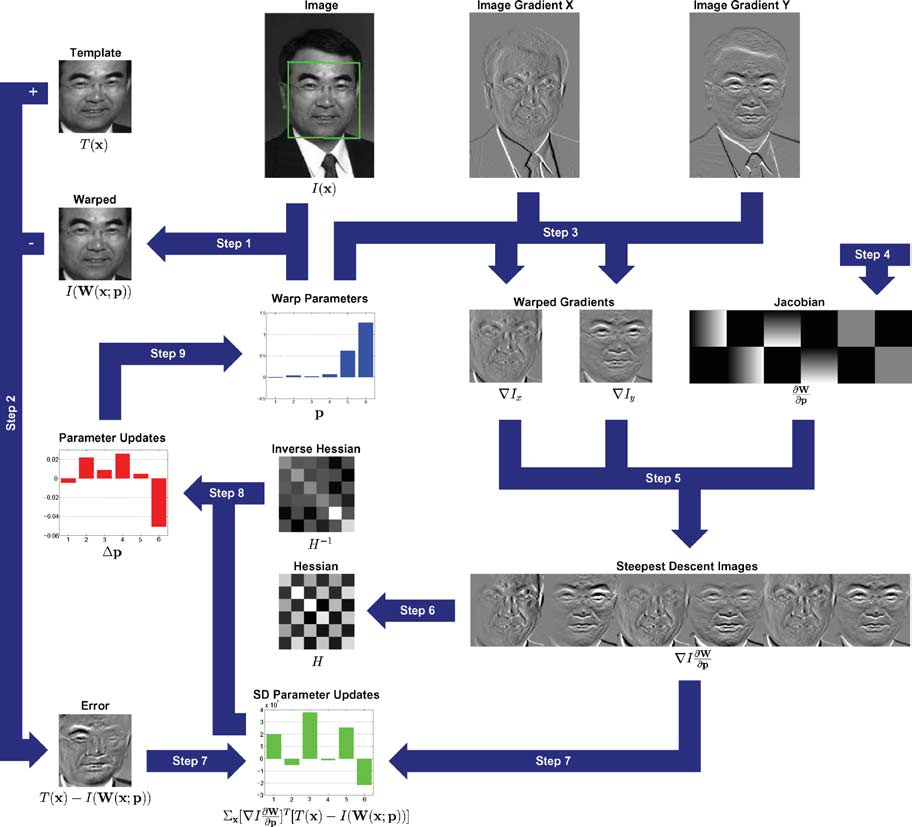
\includegraphics[width=16cm]{images/lucas_kanade_algorithm.png}
	\end{center}	
	\longcaptionsource{Przebieg algorytmu Lucasa-Kanade}{Krok 1 - wykonanie odkształcenia $W(\vec{x}, \vec{p})$ na obrazie wejściowym $I(\vec{x})$ według jego ostatniej estymacji; krok 2 - obliczenie bieżącej wartości błędu; krok 3 - wyznaczenie gradientu oraz jego odkształcenie; krok 4 - wyznaczenie macierzy Jacobiego; krok 5 - wyznaczenie $\nabla I \frac{\partial \matr{W}}{\partial \vec{p}}$; krok 6 - wyznaczenie hesjanu; krok 7 - obliczenie wartości wyrażenia $\sum\limits_{\vec{x}}(\nabla I \frac{\partial \matr{W}}{\partial \vec{p}})^T (T(\vec{x}) - I(\matr{W}(\vec{x}, \vec{p})))$; krok 8 - obliczenie zmiany wartości parametrów odkształcenia $\Delta \vec{p}$; krok 9 - uaktualnienie wektora $\vec{p}$}{\cite{Baker2004}}
\label{fig:Algorytm_Lucasa_Kanade}
\end{figure}

Znalezienie $\vec{p}$, dla którego wyrażenie \ref{equ:Algorytm_Lucasa_Kanade_Taylor} przyjmuje minimalną wartość sprowadza się do rozwiązania problemu najmniejszych kwadratów metodą Gaussa-Newtona \cite{Baker2004}. W tym celu wyznacza się jego pochodną cząstkową ze względu na $\Delta \vec{p}$ oraz porównuje się ją do zera. Po przekształceniach:
\begin{equation}
\label{equ:Algorytm_Lucasa_Kanade_Gauss_Newton}
	\Delta \vec{p} = H^{-1} \sum\limits_{\vec{x}}(\nabla I \frac{\partial \matr{W}}{\partial \vec{p}})^T (T(\vec{x}) - I(\matr{W}(\vec{x}, \vec{p})))
\end{equation}

\begin{equation}
\label{equ:Algorytm_Lucasa_Kanade_hesjan}
	H = \sum\limits_{\vec{x}}(\nabla I \frac{\partial \matr{W}}{\partial \vec{p}})^T (\nabla I \frac{\partial \matr{W}}{\partial \vec{p}})
\end{equation}

\noindent
gdzie:
\begin{conditions}
	H & aproksymacja hesjanu według metody Gaussa-Newtona \\
\end{conditions}

Cały algorytm sprowadza się do iteracyjnego wyznaczania równań \ref{equ:Algorytm_Lucasa_Kanade_Gauss_Newton} i \ref{equ:Algorytm_Lucasa_Kanade_podstawienie}. Realizację jego poszczególnych etapów przedstawiono na rysunku \ref{fig:Algorytm_Lucasa_Kanade}. Wykonanie pojedynczej iteracji ma złożoność obliczeniową $O(n^2 N + n^3)$, gdzie $N$ to liczba pikseli wzorca $T$, a $n$ to liczba parametrów odkształcenia \cite{Baker2004}.

Sam algorytm Lucasa-Kanade może być w zasadzie jedynie metodą wyznaczania gęstego przepływu optycznego \cite{Yilmaz2006}. Z drugiej strony wiadomo, że pewne punkty obrazu lepiej nadają się do realizacji zadania śledzenia obiektu niż inne \cite{Tomasi1991} - dla punktów leżących na krawędziach ujawnia się problem apertury (rozdział \ref{subsec:Ruch_w_sekwencji_obrazow}), natomiast 
punkty leżące wewnątrz obszarów o stałej intensywności nie dostarczają żadnej informacji o ruchu. W publikacji \cite{Tomasi1991} zaproponowano metodę wyznaczenia optymalnych punktów charakterystycznych oraz ich śledzenia z wykorzystaniem algorytmu Lucasa-Kanade, nazywaną \textbf{algorytmem Kanade-Lucasa-Tomasi} (ang. \textit{Kanade-Lucas-Tomasi tracker}, w skrócie \textit{KLT}).

\textit{KLT} w odróżnieniu od podstawowego algorytmu Lucasa-Kanade nie śledzi pojedynczych punktów, ale wybrane okna obrazu. Pozwala to zwiększenie odporności na szum oraz zmniejszenie prawdopodobieństwa błędnego rozpoznania punktu na kolejnym obrazie \cite{Tomasi1991}. Z drugiej strony, nie wszystkie piksele należące do konkretnego okna muszą poruszać się w jednakowy sposób (np. jeśli  okno obejmuje obszar na granicy dwóch przysłaniających się obiektów), z czym wiążą się dwa problemy: po pierwsze - jak stwierdzić, czy śledzone jest to samo okno, jeżeli jego zawartość zmienia się w czasie; po drugie - jak na podstawie informacji o prędkościach poszczególnych pikseli wnioskować o przemieszczeniu całego okna \cite{Tomasi1991}. Pierwszy problem można rozwiązać sprawdzając, jak bardzo okno zmienia się pomiędzy kolejnymi klatkami, oraz, ewentualnie, odrzucając je, jeśli zmiana jest zbyt duża. Rozwiązaniem drugiego problemu jest wprowadzenie bardziej skomplikowanego modelu zmiany okna (jak np. przekształcenia afiniczne), jednak tworzy to ryzyko nadokreślenia całego zagadnienia, ze względu na częste występowanie w sekwencjach obrazów obiektów sztywnych \cite{Tomasi1991}. Z tego powodu \textit{KLT} operuje na małych oknach, dla których wyznacza się jedynie wektor przemieszczenia, zaś każda występująca pomiędzy dwoma kolejnymi instancjami okna rozbieżność nie opisana przez niego traktowana jest jako błąd \cite{Tomasi1991}. W skutek przyjęcia założenia o małych rozmiarach okien, oryginalny algorytm \textit{KLT} nie radzi sobie w przypadku dużych przemieszczeń punktów pomiędzy klatkami. 

Przyjmując oznaczenia:
\begin{equation}
\label{equ:Algorytm_Lucasa_Kanade_Tomasi_oznaczenia}
	J(\vec{x}) = I(x, y, t + \tau)
\end{equation}

\noindent
gdzie:
\begin{conditions}
	\vec{x} & wektor współrzędnych piksela $\vec{x} = (x, y)$ \\
	I(x,y,t) & wartość piksela na obrazie $I$ o współrzędnych $(x,y)$ w chwili $t$ \\
	\tau & interwał czasowy pomiędzy dwoma kolejnymi klatkami \\
\end{conditions}

Model przemieszczenia punktu pomiędzy klatkami można zdefiniować następująco:
\begin{equation}
\label{equ:Algorytm_Lucasa_Kanade_Tomasi_model}
	J(\vec{x}) = I(\vec{x} - \vec{d}) + n(\vec{x})
\end{equation}

\noindent
gdzie:
\begin{conditions}
	\vec{d} & wektor przemieszczenia punktu $\vec{d} = (\xi, \eta)$ \\
	I(\vec{x}) & Wartość piksela na obrazie $I$ o współrzędnych $\vec{x}$ w chwili $t$ \\
\end{conditions}

Z równania \ref{equ:Algorytm_Lucasa_Kanade_Tomasi_model} należy wyznaczyć wektor przemieszczenia $\vec{d}$ tak, aby zminimalizować błąd dopasowania:
\begin{equation}
\label{equ:Algorytm_Lucasa_Kanade_Tomasi_blad_dopasowania}
	\epsilon = \int_W (I(\vec{x} - \vec{d}) - J(\vec{x}))^2 w \, d\vec{x}
\end{equation}

\noindent
gdzie:
\begin{conditions}
	w & współczynnik wagowy \\
\end{conditions}

Współczynnik wagowy $w$ może być stały i wynosić $1$ lub może przyjmować wartości zgodnie z rozkładem Gaussa, w celu podkreślenia wagi centralnej części okna \cite{Tomasi1991}. Jak widać postać równania \ref{equ:Algorytm_Lucasa_Kanade_Tomasi_blad_dopasowania} jest analogiczna do bazowego równania klasycznego algorytmu Lucasa-Kanade \ref{equ:Algorytm_Lucasa_Kanade_cel}. Całe zadanie śledzenia jest wykonywane poprzez jego zastosowanie dla punktów reprezentujących środki wybranych okien.

W algorytmie \textit{KLT} zdefiniowano również metodę doboru okien dobrze nadających się do zastosowania w zadaniu śledzenia. Opiera się ona na formalnym powiązaniu właściwości macierzy $H$ z równania \ref{equ:Algorytm_Lucasa_Kanade_Gauss_Newton} dla danego punktu z właściwościami jego otoczenia \cite{Tomasi1991}. Po pierwsze, z równania \ref{equ:Algorytm_Lucasa_Kanade_Gauss_Newton} wynika wprost, że aby śledzenie było możliwe macierz $H$ musi być niezdegenerowana, w związku z czym jej wartości własne $\lambda_1$ i $\lambda_2$ muszą być większe od poziomu szumu występującego na obrazie \cite{Tomasi1991}. Po drugie, całe zadanie powinno być dobrze uwarunkowane, co oznacza, że wartości własne $\lambda_1$ i $\lambda_2$ nie powinny znacznie się od siebie różnić \cite{Tomasi1991}.

Istnieją trzy możliwe przypadki wzajemnych relacji wartości własnych macierzy $H$:
\begin{enumerate}
	\item $\lambda_1 \gg \lambda_2$ lub $\lambda_1 \ll \lambda_2$ - otoczenie punktu stanowi wzór jednokierunkowy (krawędź) i nie jest odpowiednie do śledzenia, ze względu na problem apertury (rozdział \ref{sec:Analiza_ruchu}).
	\item $\lambda_1 \approx \lambda_2 \approx 0$ - otoczenie punktu jest obszarem o stałej intensywności i nie jest odpowiednie do śledzenia, ponieważ  nie przechowuje informacji o ruchu
	\item $\lambda_1 \approx \lambda_2 \gg 0$ - otoczenie punktu jest zróżnicowane teksturowo (narożniki, wzór pieprz-sól) i dobrze nadaje się do zadania śledzenia
\end{enumerate}

W praktyce, jeżeli mniejsza wartość własna spełnia założenie o przewyższaniu poziomu szumu, cała macierz $H$ jest również dobrze uwarunkowana, co wynika z faktu ograniczenia wartości pikseli do dozwolonego przedziału \cite{Tomasi1991}. Warunek służący do poszukiwania okien odpowiednich do śledzenia można zdefiniować następująco:
\begin{equation}
\label{equ:Algorytm_Lucasa_Kanade_Tomasi_poszukiwanie_punktow}
	\min (\lambda_1, \lambda_2) > \lambda
\end{equation}

\noindent
gdzie:
\begin{conditions}
	\lambda & wartość progowa \\
\end{conditions}

Wartość progową $\lambda$ można wyznaczyć poprzez uśrednienie wyników pomiarów wartości własnych macierzy $H$ dla arbitralnie wybranych obszarów o stałej jasność (dolna granica) oraz obszarów zróżnicowanych teksturowo (górna granica) \cite{Tomasi1991}.

\subsection{Śledzenie z wykorzystaniem cech obiektu}
\label{subsec:Sledzenie_z_wykorzystaniem_cech}